
\chapter{Building Blocks} \label{BuildingBlocks}

Building blocks are layered on top of channels. Most of them do not even need a
channel, all they need is a class that implements interface {\tt Transport} (channels
do). This enables them to work on any type of group transport that obeys this
interface.  Building blocks can be used instead of channels whenever a higher-level
interface is required. Whereas channels are simple socket-like constructs, building
blocks may offer a far more sophisticated interface. In some cases, building blocks
offer access to the underlying channel, so that -- if the building block at hand does
not offer a certain functionality -- the channel can be accessed directly.  Building
blocks are located in the {\tt org.javagroups.blocks} package. Only the ones that are
relevant for application programmers are discussed below. For a more detailed
description and for architecture and implementation details refer to the Programmer's
Guide.



  \section{PullPushAdapter} \label{PullPushAdapter}

  This class is a converter (or adapter, as used in \cite{Gamma:1995}) between the
  pull-style of actively receiving messages from the channel and the push-style where
  clients register a callback which is invoked whenever a message has been
  received. Clients of a channel do not have to allocate a separate thread for
  message reception.

  A {\tt PullPushAdapter} is always created on top of a class that implements
  interface {\tt Transport} (e.g. a channel). Clients interested in being called when
  a message is received can register with the {\tt PullPushAdapter} using method {\tt
  setListener()}. They have to implement interface {\tt MessageListener}, whose {\tt
  receive()} method will be called when a message arrives. When a client is
  interested in getting view, suspicion messages and blocks, then it must
  additionally register as a {\tt MembershipListener} using method {\tt
  setMembershipListener()}. Whenever a view, suspicion or block is received, the
  corresponding method will be called.

  Upon creation, an instance of {\tt PullPushAdapter} creates a thread which
  constantly calls the {\tt receive()} method of the underlying {\tt Transport}
  instance, blocking until a message is available. When a message is received, if
  there is a registered message listener, its {\tt receive()} method will be called.

  As this class does not implement interface {\tt Transport}, but merely uses it
  for receiving messages, an underlying object has to be used to send messages
  (e.g. the channel on top of which an object of this class resides). This is shown
  in fig. \ref{PullPushAdapterFig}.


  \begin{figure}[htb]
    \center{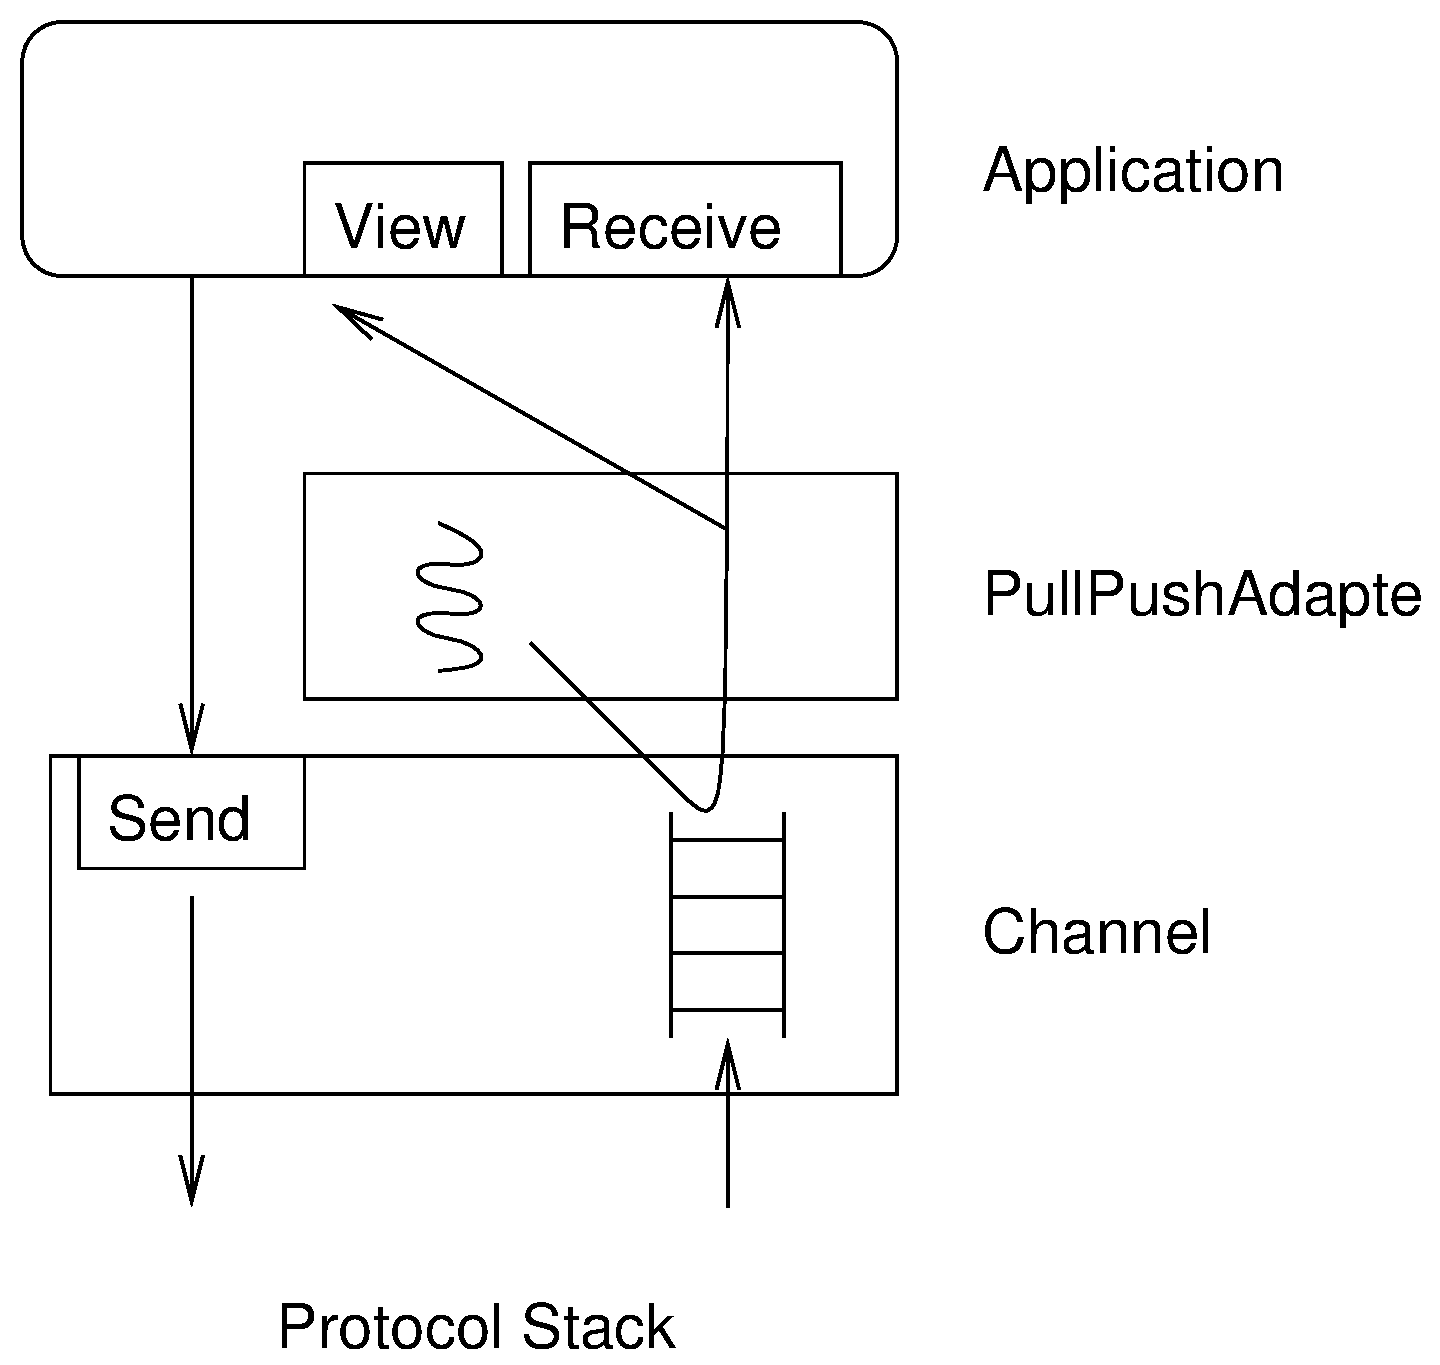
\epsfig{file=figs/PullPushAdapter.eps,width=.35\textwidth}}
    \caption{Class {\tt PullPushAdapter}}
    \label{PullPushAdapterFig}
  \end{figure}

  As is shown, the thread constantly pulls messages from the channel and forwards
  them to the registered listeners. An application thus does not have to actively pull
  for messages, but the {\tt PullPushAdapter} does this for it. Note however, that
  the application has to {\em directly} access the channel if it wants to {\em send}
  a message.



    \subsection{Example}

    This section shows sample code for using a {\tt PullPushAdapter}. The example has
    been shortened for readability (error handling has been removed).

    \begin{small}
    \begin{verbatim}

    public class PullPushTest implements MessageListener {
        Channel          channel;
        PullPushAdapter  adapter;
        byte[]           data="Hello world".getBytes();
        String           props; // fetch properties

        public void receive(Message msg) {
            System.out.println("Received msg: " + msg);
        }

        public void start() throws Exception {
            channel=new JChannel(props);
            channel.connect("PullPushTest");
            adapter=new PullPushAdapter(channel);
            adapter.setListener(this);
        
            for(int i=0; i < 10; i++) {
                System.out.println("Sending msg #" + i);
                channel.send(new Message(null, null, data));
                Thread.currentThread().sleep(1000);
            }
            adapter.stop();
            channel.close();
        }


        public static void main(String args[]) {
            try {
                new PullPushTest().start();
            }
            catch(Exception e) { /* error */ }
        }
    }
    \end{verbatim}
    \end{small}

    First a channel is created and connected to. Then an instance of {\tt
    PullPushAdapter} is created with the channel as argument. The constructor of {\tt
    PullPushAdapter} starts its own thread which continually reads on the
    channel. Then the {\tt MessageListener} is set, which causes all messages received
    on the channel to be sent to {\tt receive()}. Then a number of messages are sent
    via the channel to the entire group. As group messages are also received by the
    sender, the {\tt receive()} method will be called every time a message is
    received. Finally the {\tt PullPushAdapter} is stopped and the channel
    closed. Note that explicitly stopping the {\tt PullPushAdapter} is not actually
    necessary, a closing the channel would cause the {\tt PullPushAdapter} to
    terminate anyway.

    Note that, compared to the pull-style example, push-style message reception is
    considerably easier (no separate thread management) and requires less code to
    program.




  \section{MessageDispatcher} \label{MessageDispatcher}
	
  Channels are simple patterns to {\em asynchronously} send a receive
  messages. However, a significant number of communication patterns in group
  communication require {\em synchronous communication}. For example, a sender would
  like to send a message to the group and wait for all responses. Or another
  application would like to send a message to the group and wait only until the
  majority of the receivers have sent a response, or until a timeout occurred.

  {\tt MessageDispatcher} offers a combination of the above pattern with other
  patterns. It provides synchronous (as well as asynchronous) message sending with
  request-response correlation, e.g. matching responses with the original request. It
  also offers push-style message reception (by internally using the {\tt
  PullPushAdapter}).

  An instance of {\tt MessageDispatcher} is created with a channel as argument. It
  can now be used in both {\em client and server role}: a client sends requests and
  receives responses and a server receives requests and send responses. {\tt
  MessageDispatcher} allows a application to be both at the same time. To be able to
  serve requests, the {\tt RequestHandler.handle()} method has to be implemented:

  \begin{small}
  \begin{verbatim}
  Object handle(Message msg);
  \end{verbatim}
  \end{small}

  The {\tt handle()} method is called any time a request is received. It must return
  a return value (must be serializable, but can be null) or throw an exception. The
  return value will be returned to the sender (as a null response, see below). The
  exception will also be propagated to the requester.

  The two methods to send requests are:

  \begin{small}
  \begin{verbatim}
  public RspList castMessage(Vector dests, Message msg, int mode, long timeout);
  public Object sendMessage(Message msg, int mode, long timeout) throws TimeoutException;
  \end{verbatim}
  \end{small}

  The {\tt castMessage()} method sends a message to all members defined in {\tt
  dests}. If {\tt dests} is null the message will be sent to all members of the
  current group. Note that a possible destination set in the message will be
  overridden. If a message is sent synchronously then the {\tt timeout} argument
  defines the maximum amount of time in milliseconds to wait for the responses.

  The {\tt mode} parameter defines whether the message will be sent synchronously or
  asynchronously. The following values are valid (from {\tt org.javagroups.blocks.GroupRequest}):

  \begin{description}
  \item[GET\_FIRST] Returns the first response received.
  \item[GET\_ALL] Waits for all responses (minus the ones from suspected members)
  \item[GET\_MAJORITY] Waits for a majority of all responses (relative to the group size)
  \item[GET\_ABS\_MAJORITY] Waits for the majority (absolute, computed once)
  \item[GET\_N] Wait for n responses (may block if n > group size)
  \item[GET\_NONE] Wait for no responses, return immediately (non-blocking). This
                   make the call asynchronous.
  \end{description}

  The {\tt sendMessage()} method allows an application programmer to send a unicast
  message to a receiver and optionally receive the response. The destination of the
  message has to be non-null (valid address of a receiver). The {\tt mode} argument
  is ignored (it is by default set to {\tt GroupRequest.GET\_FIRST}) unless it is set
  to {\tt GET\_NONE} in which case the request becomes asynchronous, ie. we will not
  wait for the response.


  One advantage of using this building block is that failed members are removed from
  the set of expected responses. For example, when sending a message to 10 members and
  waiting for all responses, and 2 members crash before being able to send
  a response, the call will return with 8 valid responses and 2 marked as failed. The
  return value of {\tt castMessage()} is a {\tt RspList} which contains all responses
  (not all methods shown):

  \begin{small}
  \begin{verbatim}
  public class RspList {
      public boolean isReceived(Address sender);
      public int     numSuspectedMembers();
      public Vector  getResults();
      public Vector  getSuspectedMembers();
      public boolean isSuspected(Address sender);
      public Object  get(Address sender);
      public int     size();
      public Object  elementAt(int i) throws ArrayIndexOutOfBoundsException;
  }
  \end{verbatim}
  \end{small}

  Method {\tt isReceived()} checks whether a response from {\tt sender} has already
  been received. Note that this is only true as long as no response has yet been
  received, and the member has not been marked as failed. {\tt numSuspectedMembers()}
  returns the number of members that failed (e.g. crashed) during the wait for
  responses. {\tt getResults()} returns a list of return values. {\tt get()} returns
  the return value for a specific member.


    \subsection{Example}

    This section describes an example of how to use a {\tt MessageDispatcher}.

    \begin{small}
    \begin{verbatim}
  public class MessageDispatcherTest implements RequestHandler {
      Channel            channel;
      MessageDispatcher  disp;
      RspList            rsp_list;
      String             props; // to be set by application programmer

      public void start() throws Exception {
          channel=new JChannel(props);
          disp=new MessageDispatcher(channel, null, null, this);
          channel.connect("MessageDispatcherTestGroup");

          for(int i=0; i < 10; i++) {
              Util.sleep(100);
              System.out.println("Casting message #" + i);
              rsp_list=disp.castMessage(null,
                                        new Message(null, null, new String("Number #" + i)),
                                        GroupRequest.GET_ALL, 0);
              System.out.println("Responses:\n" +rsp_list);
          }
          channel.close();
          disp.stop();
      }

      public Object handle(Message msg) {
          System.out.println("handle(): " + msg);
          return new String("Success !");
      }

      public static void main(String[] args) {
          try {
              new MessageDispatcherTest().start();
          }
          catch(Exception e) {
              System.err.println(e);
          }
      }
  }
  \end{verbatim}
  \end{small}

  The example starts with the creation of a channel. Next, an instance of {\tt
  MessageDispatcher} is created on top of the channel. Then the channel is
  connected. The {\tt MessageDispatcher} will from now on send requests, receive
  matching responses (client role) and receive requests and send responses (server
  role).

  We then send 10 messages to the group and wait for all responses. The {\tt timeout}
  argument is 0, which causes the call to block until all responses have been
  received.

  The {\tt handle()} method simply prints out a message and returns a string.

  Finally both the {\tt MessageDispatcher} and channel are closed.

        

  \section{RpcDispatcher} \label{RpcDispatcher}

  This class is derived from {\tt MessageDispatcher}. It allows a programmer to invoke
  remote methods in all (or single) group members and optionally wait for the return
  value(s). An application will typically create a channel and layer the {\tt
  RpcDispatcher} building block on top of it, which allows it to dispatch remote
  methods (client role) and at the same time be called by other members (server
  role).

  Compared to {\tt MessageDispatcher}, no {\tt handle()} method needs to be
  implemented. Instead the methods to be called can be placed directly in the class
  using regular method definitions (see example below). The invoke remote method
  calls (unicast and multicast) the following methods are used (not all methods
  shown):

  \begin{small}
  \begin{verbatim}
  public RspList callRemoteMethods(Vector dests, String method_name, int mode, long timeout;
  public RspList callRemoteMethods(Vector dests, String method_name, Object arg1, 
				   int mode, long timeout);
  public Object callRemoteMethod(Address dest, String method_name, int mode, long timeout);
  public Object callRemoteMethod(Address dest, String method_name, Object arg1,
                                 int mode, long timeout);
  \end{verbatim}
  \end{small}

  The family of {\tt callRemoteMethods()} is invoked with a list of receiver
  addresses. If null, the method will be invoked in all group members (including the
  sender). Each call takes the name of the method to be invoked and the {\tt mode}
  and {\tt timeout} parameters, which are the same as for {\tt
  MessageDispatcher}. Additionally, each method takes zero or more parameters: there
  are {\tt callRemoteMethods()} methods with up to 3 arguments. As shown in the
  example above, the first 2 methods take zero and one parameters respectively.

  The family of {\tt callRemoteMethod()} methods takes almost the same parameters,
  except that there is only one destination address instead of a list. If the {\tt
  dest} argument is null, the call will fail.
  
  If a sender needs to use more than 3 arguments, it can use the generic versions of
  {\tt callRemoteMethod()} and {\tt callRemoteMethods()} which use a {\tt
  MethodCall}\footnote{See the Programmer's Guide and the Javadoc documentation for
  more information about this class.}  instance rather than explicit arguments.

  Java's Reflection API is used to find the correct method in the receiver according
  to the method name and number and types of supplied arguments. There is a runtime
  exception if a method cannot be resolved.

    \subsection{Example}

    The code below shows an example:

    \begin{small}
    \begin{verbatim}
  public class RpcDispatcherTest {
      Channel            channel;
      RpcDispatcher      disp;
      RspList            rsp_list;
      String             props; // set by application

      public int print(int number) throws Exception {
          return number * 2;
      }

      public void start() throws Exception {
          channel=new JChannel(props);
          disp=new RpcDispatcher(channel, null, null, this);
          channel.connect("RpcDispatcherTestGroup");

          for(int i=0; i < 10; i++) {
              Util.sleep(100);
              rsp_list=disp.callRemoteMethods(null, "print", new Integer(i), GroupRequest.GET_ALL, 0);
              System.out.println("Responses: " +rsp_list);
          }
          channel.close();
          disp.stop();
      }

      public static void main(String[] args) {
          try {
              new RpcDispatcherTest().start();
          }
          catch(Exception e) {
              System.err.println(e);
          }
      }
  }
    \end{verbatim}
    \end{small}

    Class {\tt RpcDispatcher} defines method {\tt print()} which will be called
    subsequently. The entry point {\tt start()} method creates a channel and an {\tt
    RpcDispatcher} which is layered on top. Method {\tt callRemoteMethods()} then
    invokes the remote {\tt print()} method in all group members (also in the
    caller). When all responses have been received, the call returns and the
    responses are printed.

    As can be seen, the {\tt RpcDispatcher} building block reduces the amount of code
    that needs to be written to implement RPC-based group communication applications
    by providing a higher abstraction level between the application and the primitive
    channels.



  \section{DistributedHashtable} \label{DistributedHashtable}

  A {\tt DistributedHashtable} is derived from {\tt java.util.Hashtable} and allows
  to create several instances of hashtables in different processes. All of these
  instances have exactly the same state at all times. When creating such an instance,
  a group name determines which group of hashtables will be joined. The new instance
  will then query the state from existing members and update itself before starting
  to service requests. If there are no existing members, it will simply start with an
  empty state.

  Modifications such as {\tt put()}, {\tt clear()} or {\tt remove()} will be
  propagated in orderly fashion to all replicas. Read-only requests such as {\tt
  get()} will only be sent to the local copy.

  Since both keys and values of a hashtable will be sent across the network as
  copies, both of them have to be serializable. This allows for example to register
  remote RMI objects with any local instance of a hashtable, which can subsequently
  be looked up by another process which can then invoke remote methods (remote RMI
  objects are serializable). Thus, a distributed naming and registration service can
  be built in just a couple of lines.

  A {\tt DistributedHashtable} allows to register for notifications, e.g. when a new
  item is set, or an existing one removed. All registered listeners will notified
  when such an event occurs. Notification is always local; for example in the case of
  removing an element, first the element is removed in all replicas, which then
  notify their listener(s) of the removal (after the fact).

  {\tt DistributedHashtable} allow members in a group to share common state across
  process and machine boundaries.



  \section{ReplicatedHashtable}

  {\tt ReplicatedHashtable} provides exactly the same methods as as {\tt
  DistributedHashtable}. However, it is implemented differently. Whereas the latter
  uses synchronous remote group method invocation (similar to {\tt RpcDispatcher}),
  the former uses asynchronous communication to keep the replicas up-to-date.
  


  \section{DistributedTree}

  Similar to {\tt DistributedHashtable} this class also provides replication of a
  data structure across multiple processes. However, a tree structure instead of a
  hashtable is replicated by {\tt DistributedTree}. Updates are multicast to all group
  members reliably and in the same order using the underlying channel.

  The tree consists of a root and zero or more child nodes. Each node can be either
  another subtree, or a leaf node. A node has a name and a value. The value can be
  any object that is serializable. A node in the tree is identified by concatenating
  all nodes from the root to it, separated with {\tt '/'} characters, e.g. 

  {\tt /a/b/c}.

  New nodes can be added dynamically. Existing nodes (also entire subtrees) can be
  removed. Values can be attached to an existing node. Whenever the tree is modified
  events will be sent for which listeners can register. Listeners have to implement
  interface {\tt DistributedTreeListener}:

  \begin{small}
  \begin{verbatim}
  public interface DistributedTreeListener {
      void nodeAdded(String fqn, Serializable element);
      void nodeRemoved(String fqn);
      void nodeModified(String fqn, Serializable old_element, Serializable new_element);
  }
  \end{verbatim}
  \end{small}

  The methods provided by {\tt DistributedTree} are listed below (not all methods
  shown):

  \begin{small}
  \begin{verbatim}
  public class DistributedTree {
       public void         add(String fqn);
       public void         add(String fqn, Serializable element);
       public void         remove(String fqn);
       public boolean      exists(String fqn);
       public Serializable get(String fqn);
       public void         set(String fqn, Serializable element);
       public Vector       getChildrenNames(String fqn);
  }
  \end{verbatim}
  \end{small}

  The two {\tt add()} methods add a new node. The first method assigns no value to
  the node, whereas the second does. Note that it does not matter whether or not
  parent nodes exists: an addition of {\tt "/a/b/c/d"} to a tree {\tt "/a/b"} would
  create nodes {\tt "/a/b/c"} and {\tt "/a/b/c/d"}. However, if a value was given, it
  would be assigned only to the latter.

  The {\tt remove()} method removes a node from the tree. If the node is a subtree
  itself, all nodes under it will be removed recursively. E.g. the removal of {\tt
  "/"} from {\tt "/a/b"} would trigger 3 {\tt nodeRemoved()} notifications: {\tt "/a/b"},
  {\tt "/a"} and {\tt "/"} (in this order)\footnote{Assuming that these are the only
  nodes in the entire tree, e.g. {\tt "/a"} has no other children}.

  The {\tt exists()} method tests whether a given node exists in the tree.

  The {\tt get()} method returns either the value associated with the given node, or
  null if the node cannot be found or there is no value attached.

  Method {\tt set()} attaches a value to a given node. It fails if the node does not
  exist. Use {\tt add(String, Serializable)} instead if the node should be created if
  not existent.

  Method {\tt getChildrenNames()} furnishes a list of the fully qualified names of
  all children nodes of a given node. This gives a programmer modest navigation
  possibilities within the tree.

  There is a demo application in {\tt org.javagroups.demos.DistributedTreeDemo}.



  \section{NotificationBus}

  This class provides notification sending and handling capability. Also, it allows
  an application programmer to maintain a local cache which is replicated by all
  instances. {\tt NotificationBus} also sits on top of a channel, however it creates
  its channel itself, so the application programmers do not have to provide their own
  channel. Notification consumers can subscribe to receive notifications by calling
  {\tt setConsumer()} and implementing interface {\tt NotificationBus.Consumer}:

  \begin{small}
  \begin{verbatim}
  public interface Consumer {
      void          handleNotification(Serializable n);
      Serializable  getCache();
      void          memberJoined(Address mbr);
      void          memberLeft(Address mbr);
  }
  \end{verbatim}
  \end{small}

  Method {\tt handleNotification()} is called whenever a notification is received
  from the channel. A notification is any object that is serializable. Method {\tt
  getCache()} is called when someone wants to retrieve our state; the state can be
  returned as a serializable object. The {\tt memberJoined()} and {\tt memberLeft()}
  callbacks are invoked whenever a member joins or leaves (or crashes).

  The most important methods of {\tt NotificationBus} are:

  \begin{small}
  \begin{verbatim}
  public class NotificationBus {
       public void setConsumer(Consumer c);
       public void start() throws Exception;
       public void stop();
       public void sendNotification(Serializable n);
       public Serializable getCacheFromCoordinator(long timeout, int max_tries);
       public Serializable getCacheFromMember(Address mbr, long timeout, int max_tries);
  }
  \end{verbatim}
  \end{small}

  Method {\tt setConsumer()} allows a consumer to register itself for notifications.

  The {\tt start()} and {\tt stop()} methods start and stop the {\tt
  NotificationBus}.

  Method {\tt sendNotification()} sends the serializable object given as argument to
  all members of the group, invoking their {\tt handleNotification()} methods on
  reception.

  Methods {\tt getCacheFromCoordinator()} and {\tt getCacheFromMember()} provide
  functionality to fetch the group state from the coordinator (first member in
  membership list) or any other member (if its address is known). They take as
  arguments a timeout and a maximum number of unsuccessful attempts until they return
  null. Typically one of these methods would be called just after creating a new {\tt
  NotificationBus} to acquire the group state. Note that if these methods are used,
  then the consumers must implement {\tt Consumer.getCache()}, otherwise the two
  methods above would always return null.
